\documentclass{beamer}
\usepackage{xeCJK}
\usepackage{graphicx}
\usepackage{xcolor}
\usepackage{setspace}

% ============= setup =============
\setCJKmainfont{Taipei Sans TC Beta}
\setCJKsansfont{Taipei Sans TC Beta}
\hypersetup{
    colorlinks=true,
    linkcolor=black,
    urlcolor=blue
}
\renewcommand{\baselinestretch}{1.25}
\usetheme{Madrid}
\usecolortheme{crane}
\setbeamertemplate{items}[circle]
\setbeamertemplate{section in toc}{\inserttocsectionnumber.~\inserttocsection}
\AtBeginSection[]{
    \begin{frame}
        \vfill
        \centering
        \begin{beamercolorbox}[sep=8pt,center,shadow=true,rounded=true]{title}
            \usebeamerfont{title}\insertsectionhead\par%
        \end{beamercolorbox}
        \vfill
    \end{frame}
}

\title{實做能力加強}
\author{temmie}
\date{}
% ============= setup =============

\begin{document}

\begin{frame}
    \titlepage
\end{frame}

\begin{frame}
    \tableofcontents
\end{frame}

\section{位元運算}

\begin{frame}
    \frametitle{為什麼要學這個?}
    \begin{itemize}
        \item 因為電腦的機制,位元運算會比一般運算更快一些
        \item 在\textbf{枚舉}這堂課上,我們會用到很多
    \end{itemize}
\end{frame}

\begin{frame}
    \frametitle{進位制}
    \begin{itemize}
        \item n 進位代表只用 n 以內的數字組成(如果超過 10 就用英文)
        \item 二進位的數字代表只用 0 和 1 組成
        \item<2-> 如果一個式子有不同進位制的數字,則會用括弧備註在右下角
        \item<2-> 例如:$17_{(10)}=10001_{(2)}$
    \end{itemize}
\end{frame}

\begin{frame}
    \frametitle{二進位轉十進位}
    \begin{itemize}
        \item 以 $10001_{(2)}$ 舉例
        \item 我們可以先把所有 2 的冪次列出來:$2^4$、$2^3$、$2^2$、$2^1$、$2^0$
        \item<2-> 和原本的二進位字串一一對應後相乘
        $1\times 2^4$、$0\times 2^3$、$0\times 2^2$、$0\times 2^1$、$1\times 2^0$
        \item<3-> 將所有數字相加
        $1\times 2^4+0\times 2^3+0\times 2^2+0\times 2^1+1\times 2^0=17$
    \end{itemize}
\end{frame}

\begin{frame}
    \frametitle{十進位轉二進位}
    \begin{itemize}
        \item 詳細作法如下圖
        \item 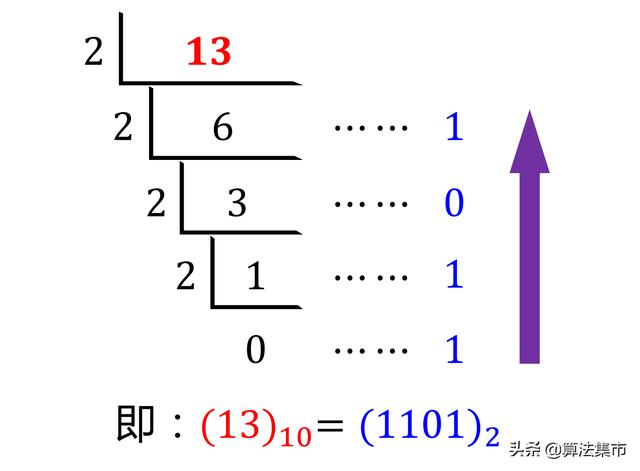
\includegraphics[width=7.0cm]{img/img_1.png}
    \end{itemize}
\end{frame}

\begin{frame}
    \frametitle{例題}
    \begin{block}{二進位制轉換}
        \href{https://zerojudge.tw/ShowProblem?problemid=a034}{題目連結}\\
        給你一個十進位的正整數 $n$,輸出 $n$ 的二進位
    \end{block}
\end{frame}

\begin{frame}
    \frametitle{位元運算的類別}
    \begin{itemize}
        \item 主要有 OR、AND、XOR、NOT
        \item 和一般的 or、and、not 不同的是,可以對數字做運算,而不是限制在布林
        \vspace{0.5cm}
        \item<2-> $AND$: 「 & 」 表示,如果兩個 bit \textbf{都是} 1 就是 1,否則為 0
        \item<2-> $OR$: 「 | 」 表示,如果兩個 bit \textbf{至少}有一個 1 就是 1,否則為 0
        \item<2-> $XOR$: 「 ^ 」 表示,如果兩個 bit \textbf{恰有}一個為 1,否則為 0
        \item<2-> $NOT$: 「 ~ 」表示,將 1 變成 0,0 變成 1
        % 記得手算真值表舉例
    \end{itemize}
\end{frame}

\begin{frame}
    \frametitle{使用位元運算}
    \begin{itemize}
        \item 難道用位元運算還要手動轉進位制? @@
        \item<2-> 在 C++ 中,直接對兩個十進位的數字做就可以了
        \item<2-> $17_{(10)} \mid 5_{(10)} = 10001_{(2)} \mid 00101_{(2)} = 10101_{(2)} = 21_{(10)}$
    \end{itemize}
\end{frame}

\begin{frame}
    \frametitle{例題}
    \begin{block}{位元運算的大雜燴}
        \href{https://codeforces.com/group/S6XjkGb6qB/contest/403070/problem/B}{題目連結}\\
        給你三個參數 $x$、$y$、$z$ ,找到 $(x \oplus (y \mid z)) \oplus (x+y)$ 的最小值\\
        其中 $\oplus$ 是 XOR 的意思,$\mid$ 是 OR 的意思
    \end{block}
    \begin{itemize}
        \item<2-> 參數數量是固定的,那就列出所有情況吧!
        \item<2-> 把六種組合各試一遍就可以了
    \end{itemize}
\end{frame}

\begin{frame}
    \frametitle{更多位元運算}
    \begin{itemize}
        \item 另外常用的位元運算有左移和右移
        \vspace{0.5cm}
        \item<2-> 左移: 「 << 」 表示,代表將所有 bit 左移 n 位
        \item<2-> 右移: 「 >> 」 表示,代表將所有 bit 右移 n 位
        \vspace{0.5cm}
        \item<3-> 例如: $17_{(10)} << 1 = 10001_{(2)} << 1 = 100010_{(2)} = 34_{(10)}$
        \item<3->你知道嗎?實際上左移就是乘上 $2^n$(右移則相反)
    \end{itemize}
\end{frame}

\section{字元轉換}

\begin{frame}
    \frametitle{Ascii}
    \begin{itemize}
        \item 我們都知道電腦是儲存 0 跟 1,並不能儲存字元
        \item 那要怎麼儲存字元呢?
        \item<2-> 只要把所有字母編碼就可以啦!
        \item<2-> 實際上我們用的字元都有一個編碼,稱為 Ascii 編碼
    \end{itemize}
\end{frame}

\begin{frame}
    \frametitle{Ascii}
    \begin{itemize}
        \item $[\ 0-9\ ]$ = 48 $\sim$ 57
        \item $[\ A-Z\ ]$ = 65 $\sim$ 90
        \item $[\ a-z\ ]$ = 97 $\sim$ 122
        \item 利用編碼的連續性,就有很多功能可以應用
    \end{itemize}
\end{frame}

\begin{frame}
    \frametitle{例題}
    \begin{block}{數字總和}
        \href{https://codeforces.com/group/S6XjkGb6qB/contest/403070/problem/C}{題目連結}\\
        你有一個數字 $n$,請你求出所有位數的總和,保證 $n$ 的位數 $\leq 10^5$
    \end{block}
    \begin{itemize}
        \item<2-> 字串很大,看起來沒辦法用 int 儲存,所以只能用 string 儲存
        \item<2-> 我們可以用 for 得到每個字元,並且\textbf{減去 '0'},就可以轉換成數字
        \item<2-> '0'(48)-'0'(48)=0,'1'(49)-'0'(48)=1
        \item<2-> '5'(53)-'0'(48)=5,'9'(57)-'0'(48)=9
    \end{itemize}
\end{frame}

\begin{frame}
    \frametitle{例題}
    \begin{block}{凱撒密碼}
        \href{https://zerojudge.tw/ShowProblem?problemid=b516}{題目連結}\\
        給你一個字串 $s$,把每個字母向後移 3 位,例如 A → D,Z → C
    \end{block}
    \begin{itemize}
        \item<2-> 我們可以將每個字母的值都加上 3
        \item<2-> 如果該字母超過 'Z' 的話就減去 26
    \end{itemize}
\end{frame}

\section{陣列運用}

\begin{frame}
    \frametitle{陣列運用}
    \begin{itemize}
        \item 陣列的用途很廣,巧妙的使用陣列可以讓時間複雜度更好
        \item 用陣列也可以實做很多好用的資料結構,並提供額外的性質
    \end{itemize}
\end{frame}

\begin{frame}
    \frametitle{vector}
    \begin{itemize}
        \item vector 可以說是更好的陣列,\textbf{可以動態的分配空間}
        \item 陣列做的事 vector 做的到,陣列不能做的事 vector 也可以做的到
        \item 缺點:可能比陣列慢一點點、大量宣告可能會吃到 MLE
    \end{itemize}
\end{frame}

\begin{frame}
    \frametitle{vector 的宣告和使用}
    vector<{\color[rgb]{1,0,0}type}> {\color[rgb]{1,0,0}name}({\color[rgb]{1,0,0}size}, {\color[rgb]{1,0,0}value});
    \begin{itemize}
        \item type 是放 vector 裡面東西的型別
        \item name 則是 vector 的名稱(接下來的介紹都用 vec 表示)
        \item (可選)size 可以放初始的陣列大小
        \item (可選)value 可以放初始值
    \end{itemize}
    \vspace{0.5cm}
    {\color[rgb]{1,0,0}name}.{\color[rgb]{1,0,0}method}({\color[rgb]{1,0,0}value1}, {\color[rgb]{1,0,0}value2}...)
    \begin{itemize}
        \item 以上為 vector 如何使用的模板
    \end{itemize}
\end{frame}


\begin{frame}
    \frametitle{vector 的資料位置}
    \begin{itemize}
        \item .begin() 代表 vector 裡第一個資料位置
        \item .end() 代表 vector 裡最後一個資料\textbf{的後一位}位置
        \item vec[i] 代表 vector 裡的第 i 個資料
        \item<2-> 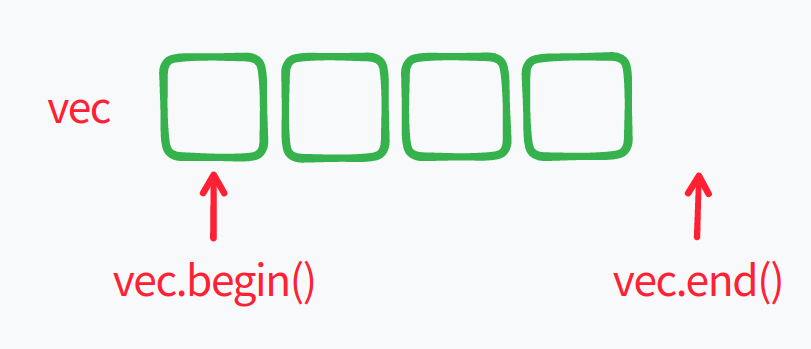
\includegraphics[width=8.0cm]{img/img_2.png}
        \item<2-> 要對整個 vector 操作丟 .begin() 跟 .end() 就好了
    \end{itemize}
\end{frame}

\begin{frame}
    \frametitle{vector 的使用}
    \begin{itemize}
        \item 以後介紹的函式,除非有特別標注,否則都為以下的方法
        \item 開始都是包含,結束則不包含
        \item 書寫的形式為 [ L, R )
        \item 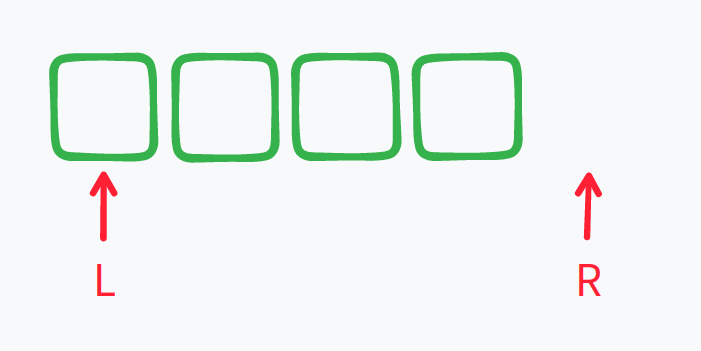
\includegraphics[width=8.0cm]{img/img_3.png}
    \end{itemize}
\end{frame}

\begin{frame}
    \frametitle{vector 的輸入方式}
    \begin{itemize}
        \item 分配好空間,並且用 cin >> [i]
        \item 不分配空間,用 vec.push\_back({\color[rgb]{1,0,0}value}) 將元素放入最後一位
        \vspace{0.5cm}
        \item 要用哪一個?如果後續沒有要操作就用第ㄧ個,否則用另一個
    \end{itemize}
\end{frame}

\begin{frame}
    \frametitle{vector 的各種常用操作}
    \begin{itemize}
        \item $O(1)$,.size(),取得 vector 的大小
        \item $O(1)$,.empty(),回傳 vector 是否為空
        \item $O(\mid size-n \mid )$,.resize({\color[rgb]{1,0,0}n}, {\color[rgb]{1,0,0}[val]})\\
        重設 vector 的大小,並設為 val(可選)
        \item $O(1)$,.pop\_back(),清除 vector 最後面的元素
        \item $O(1)$,.clear(),清空 vector
        \item $O(1)$,.front(),回傳最前面的元素
        \item $O(1)$,.back(),回傳最後面的元素
    \end{itemize}
\end{frame}

\begin{frame}
    \frametitle{vector 的各種常用操作}
    \begin{itemize}
        \item $O(n)$,*max\_element({\color[rgb]{1,0,0}L}, {\color[rgb]{1,0,0}R}),取得 [ L, R ) 的最大值
        \item $O(n)$,*min\_element({\color[rgb]{1,0,0}L}, {\color[rgb]{1,0,0}R}),取得 [ L, R ) 的最小值
        \item $O(1)$,swap({\color[rgb]{1,0,0}vec1}, {\color[rgb]{1,0,0}vec2}),將 vec1 跟 vec2 對調
        \item $O(n)$,fill({\color[rgb]{1,0,0}L}, {\color[rgb]{1,0,0}R}, {\color[rgb]{1,0,0}val}),將 [ L, R ) 設為 val
        \item $O(n \log n)$,sort({\color[rgb]{1,0,0}L}, {\color[rgb]{1,0,0}R}),將 [ L, R ) 排序
        \vspace{0.5cm}
        \item 內容很多,以知道有這些功能為主,多練習題目自然就會記起來了
        \item 特別注意,有些 $O(n)$ 不要用太多次
    \end{itemize}
\end{frame}

\begin{frame}
    \frametitle{vector 的遍歷}
    \begin{itemize}
        \item 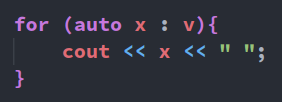
\includegraphics[width=5.0cm]{img/img_4.png}
        \item 其中 x 就會是 vector 裡的所有元素
        \item 想要改值?回想前一節講的吧!
    \end{itemize}
\end{frame}

\begin{frame}
    \frametitle{例題}
    \begin{block}{圖書館}
        \href{https://zerojudge.tw/ShowProblem?problemid=f819}{題目連結}\\
        給你 $n$ 本書,每本書都有編號 $a_i$ 和借閱日期 $b_i$\\
        如果借閱日期超過 100 天就代表逾期,每超過 1 天就要罰 5 元罰金\\
        請求出所有逾期的書的編號,以及總罰金
    \end{block}
    \begin{itemize}
        \item<2-> 我們可以把所有逾期的書都裝進 vector 裡,是不是簡單又方便呢?
    \end{itemize}
\end{frame}

\begin{frame}
    \frametitle{二維 vector 的宣告和使用}
    vector<vector<{\color[rgb]{1,0,0}type}$\textgreater\textgreater$ {\color[rgb]{1,0,0}name}({\color[rgb]{1,0,0}size1}, vector<int>({\color[rgb]{1,0,0}size2}, {\color[rgb]{1,0,0}value}))
    \begin{itemize}
        \item 以上如同 int[ ][ ]
        \item 不過實在是太長了,通常我還是會用 int[ ][ ]
    \end{itemize}
    \vspace{0.5cm}
    vector<{\color[rgb]{1,0,0}type}> {\color[rgb]{1,0,0}name}[{\color[rgb]{1,0,0}size}]
    \begin{itemize}
        \item 這也是二維陣列,不過每一項都可以是不同大小
        \item 在\textbf{圖論}這個單元我們會很常用到
    \end{itemize}
    \vspace{0.5cm}
    該學哪個?一如往常的,兩個都要學
\end{frame}

\begin{frame}
    \frametitle{二維 vector 的比較}
    \vspace{0.5cm}
    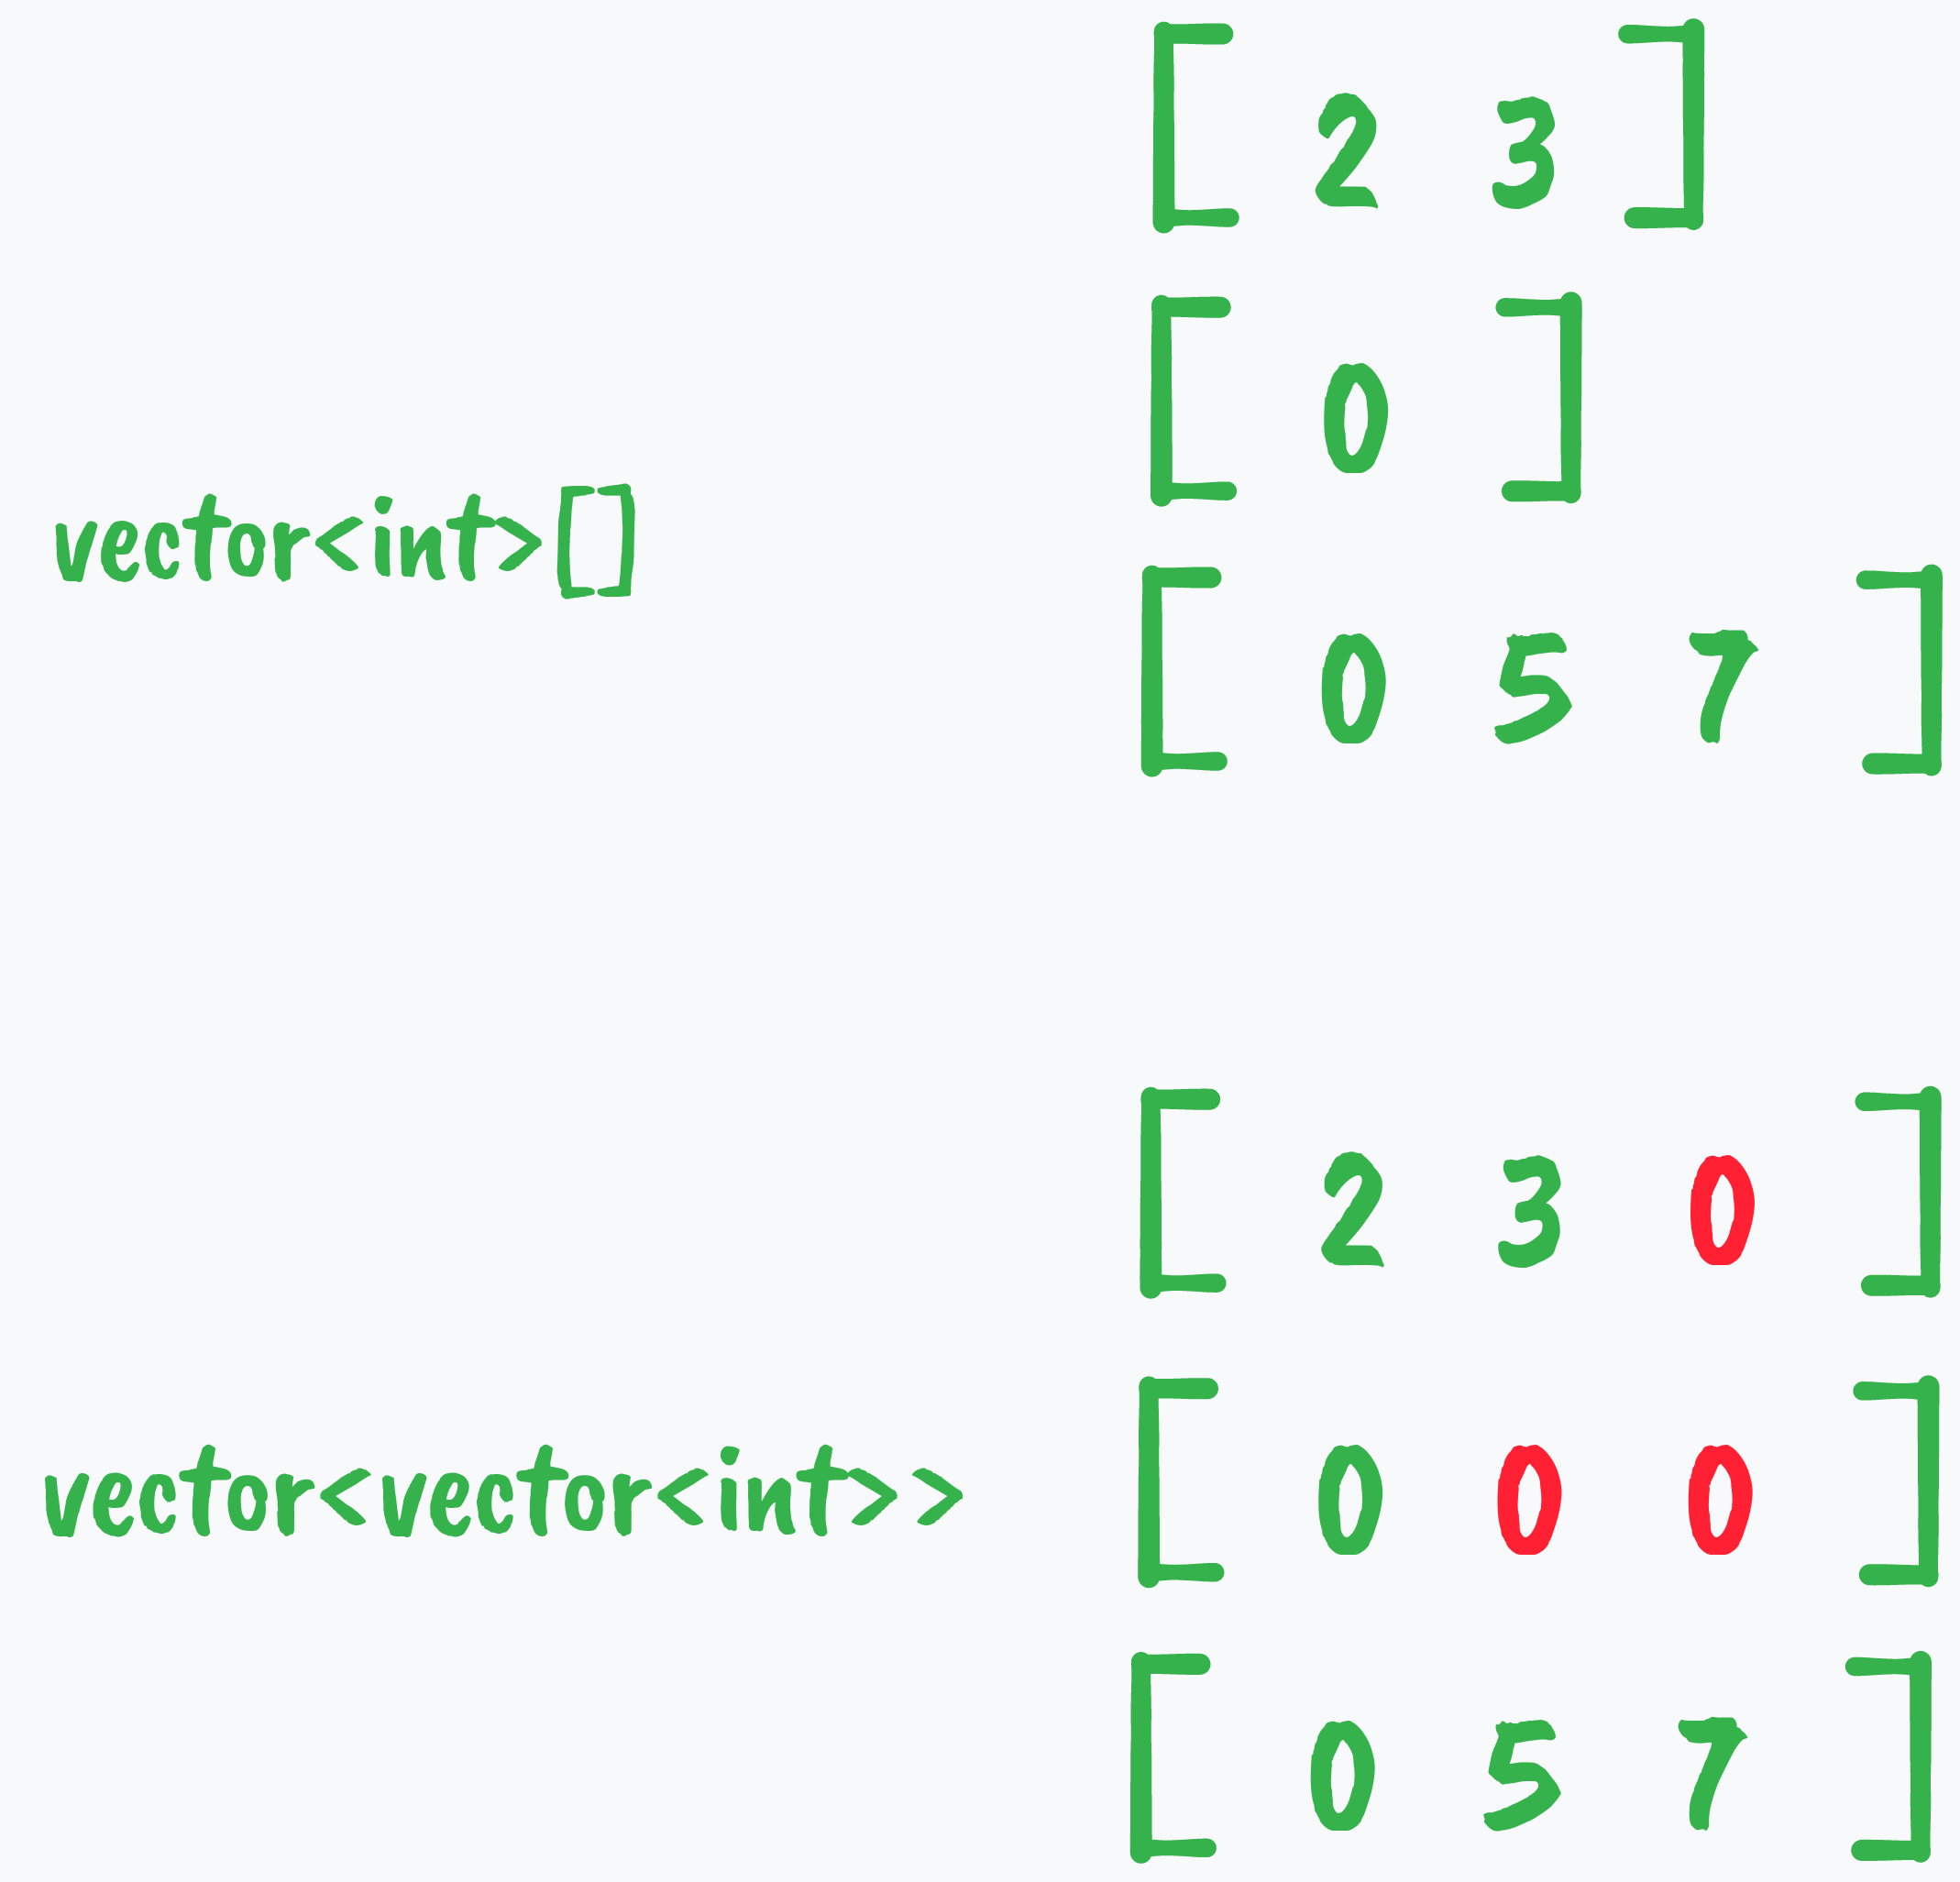
\includegraphics[width=7.0cm]{img/img_5.png}
\end{frame}

\begin{frame}
    \frametitle{例題}
    \begin{block}{vector練習}
        \href{https://toj.tfcis.org/oj/pro/575/}{題目連結}\\
        給你 $n$ 個人,並且有 $k$ 組朋友關係,由小到大輸出每個人的朋友有哪些\\
        每組朋友關係有兩個整數 $a$、$b$,代表 $a$ 和 $b$ \textbf{互相為}朋友\\
        (記得 IO 加速)
    \end{block}
    \begin{itemize}
        \item<2-> 這題其實就是圖的儲存!我們留到圖論在說
    \end{itemize}
\end{frame}

\section{區間問題}

\begin{frame}
    \frametitle{區間問題概述}
    \begin{itemize}
        \item 在競程裡面,我們有相當多的問題是有關於「區間」的
        \item 透過不同的資料結構、演算法,就可以解決這些
        \item 讓我們試著解決第一道問題
    \end{itemize}
\end{frame}

\begin{frame}
    \frametitle{例題}
    \begin{block}{區間和問題ㄧ}
        給你一個有 $n$ 個正整數的陣列 $arr$\\
        給予 $q$ 個查詢,每個查詢都有兩個正整數 $L_i$,$R_i$\\
        對於每個查詢求出 [ $L_i$, $R_i$ ] 的總和\\

        保證 $1 \leq n, q \leq 1000$
    \end{block}
    \begin{itemize}
        \item<2-> 這應該滿簡單的,對於每個查詢都直接把所有數字加起來就好
    \end{itemize}
\end{frame}

\begin{frame}
    \frametitle{例題}
    \begin{block}{區間和問題二}
        給你一個有 $n$ 個正整數的陣列 $arr$\\
        給予 $q$ 個查詢,每個查詢都有兩個正整數 $L_i$,$R_i$\\
        對於每個查詢求出 [ $L_i$, $R_i$ ] 的總和\\

        保證 $1 \leq n, q \leq 2 \times 10^5$
    \end{block}
    \begin{itemize}
        \item<2-> 和上一題看起來一模一樣,不過範圍變大了
        \item<2-> 不出意外的話,你應該吃了 TLE
        \item<3-> 讓我們分析看看問題一的時間複雜度
        \item<3-> 由於有 q 個查詢,每個查詢都有可能從 $arr_1$ 找到 $arr_n$
        \item<3-> 時間複雜度是 $O(n \times q)$,在這一題顯然不適用
    \end{itemize}
\end{frame}

\begin{frame}
    \frametitle{前綴和概念}
    \begin{itemize}
        \item 前綴和可以處理\textbf{沒有修改,只有查詢}的問題
        \item 其中每個查詢都可以在 $O(1)$ 完成
        \item 非常非常非常重要的技巧,很常出現
    \end{itemize}
\end{frame}

\begin{frame}
    \frametitle{前綴和概念}
    \begin{itemize}
        \item 
\includegraphics[width=3.0cm]{img/img_6.png}
        \item 上圖的藍色區域怎麼算呢?
        \item<2-> 只要算出正方形的面積,並且減去扇形,即可求解
        \item<2-> 讓我們看看這個概念放到陣列上會變成怎樣
    \end{itemize}
\end{frame}

\begin{frame}
    \frametitle{前綴和概念}
    \begin{itemize}
        \item 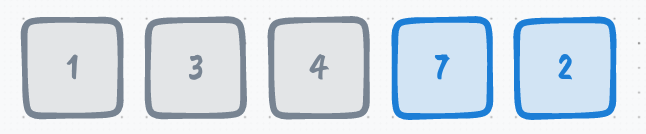
\includegraphics[width=8.0cm]{img/img_7.png}
        \item 我們可以算出所有數字的總和,然後扣除灰色的部份
        \item<2-> 嗯?這樣應該算的數字更多,因此更慢不是嗎?
        \item<2-> 實際上,我們可以儲存這些數字,要用時再扣除,這樣就很快啦!
    \end{itemize}
\end{frame}

\begin{frame}
    \frametitle{前綴和概念}
    \begin{itemize}
        \item 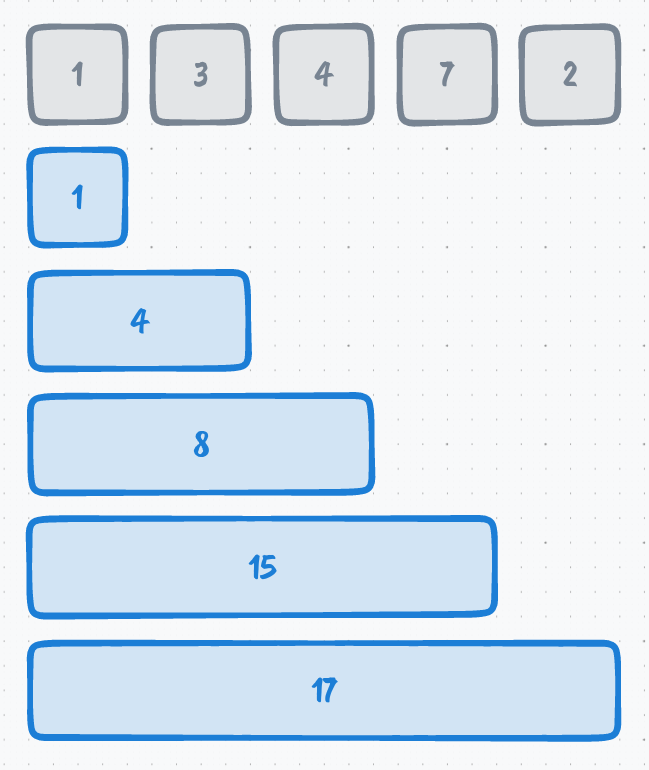
\includegraphics[width=4.5cm]{img/img_8.png}
        \item 試著把上面的藍色數值兩兩相減看看,然後觀察他們的性質吧
        \item 如果我想要獲得一個區間的和,該怎麼求得呢?
    \end{itemize}
\end{frame}

\begin{frame}
    \frametitle{前綴和概念}
    \begin{itemize}
        \item 稍微整理一下,要找到一個區間 [ L, R ] 的和
        \item 則將 [ 0, R ] - [ 0, L-1 ] 即可
        \item 而 [ 0, n ] 的值可以從 [ 0, n-1 ] + $a_n$ 得到
    \end{itemize}
\end{frame}

\begin{frame}
    \frametitle{前綴和實做}
    \begin{itemize}
        \item 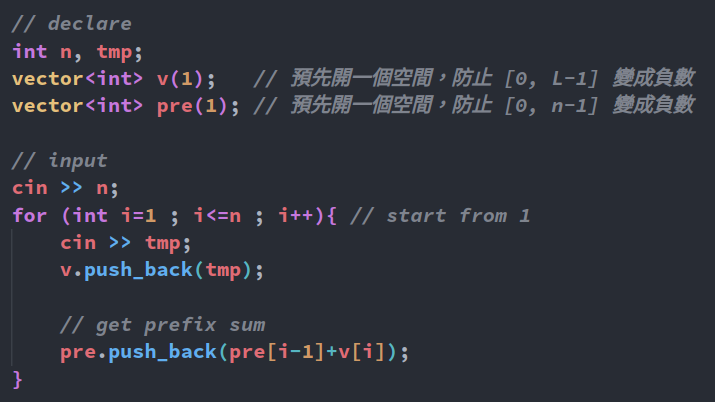
\includegraphics[width=10.0cm]{img/img_9.png}
        \item 上面這個過程叫做預處理
        \item 先把陣列建起來,後面的查詢可以用
    \end{itemize}
\end{frame}

\begin{frame}
    \frametitle{前綴和實做}
    \begin{itemize}
        \item 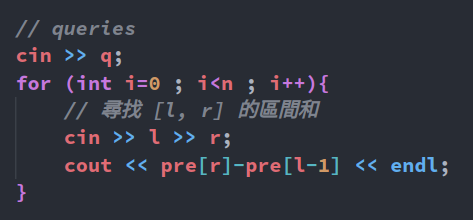
\includegraphics[width=8.0cm]{img/img_10.png}
        \item 每次查詢都直接拿陣列裡面的值,時間複雜度為 $O(1)$
    \end{itemize}
\end{frame}

\begin{frame}
    \frametitle{額外問題}
    \begin{block}{區間和問題三}
        \href{https://cses.fi/problemset/task/1652}{題目連結}\\
        給你一個 $n \times n$ 大小的森林,森林的每一個座標都是空地或是樹\\
        給予 $q$ 個查詢,每個查詢包含 $y_{1_i}$、$x_{1_i}$、$y_{2_i}$、$x_{2_i}$
        對於每個查詢輸出該範圍有多少顆樹
    \end{block}
    \begin{itemize}
        \item 請你想想看,如何運用同樣的概念做二維的區間查詢呢?
        \item<2-> 我們一樣儲存 $(0, 0)$ 到 $(x, y)$ 的區間和
        \item<2-> 並用相同的\textbf{扣除不需要的範圍}的概念
    \end{itemize}
\end{frame}

\begin{frame}
    \frametitle{額外問題}
    \begin{itemize}
        \item 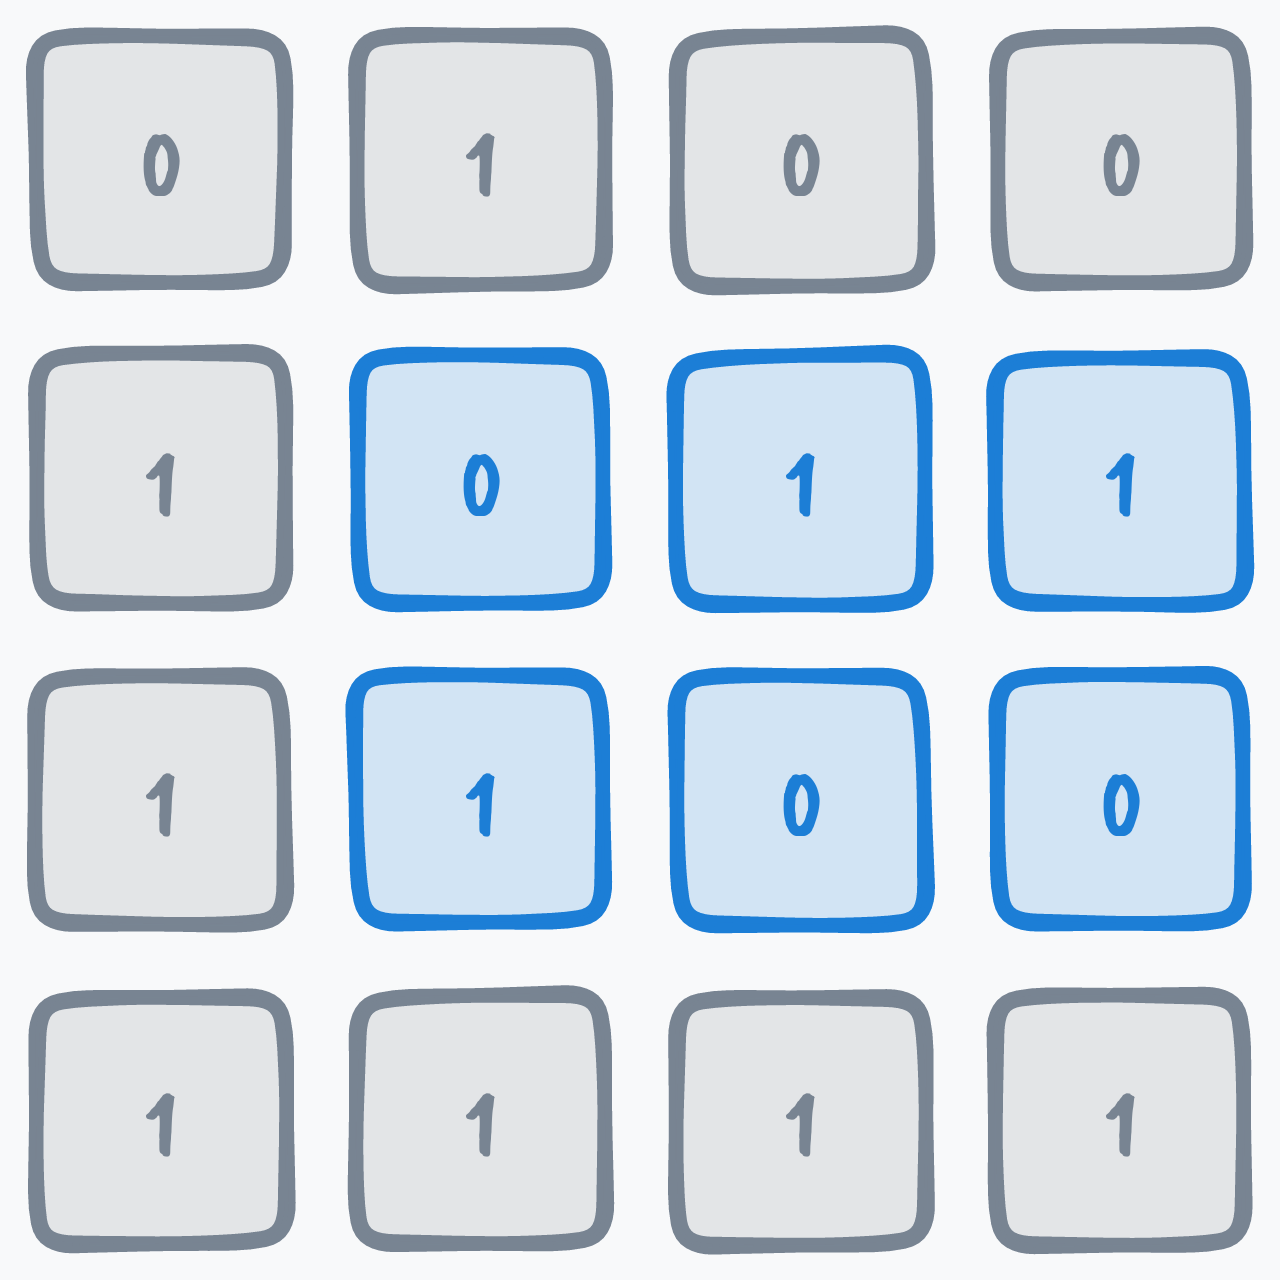
\includegraphics[width=6.0cm]{img/img_11.png}
    \end{itemize}
\end{frame}

\begin{frame}
    \frametitle{額外問題}
    \begin{itemize}
        \item 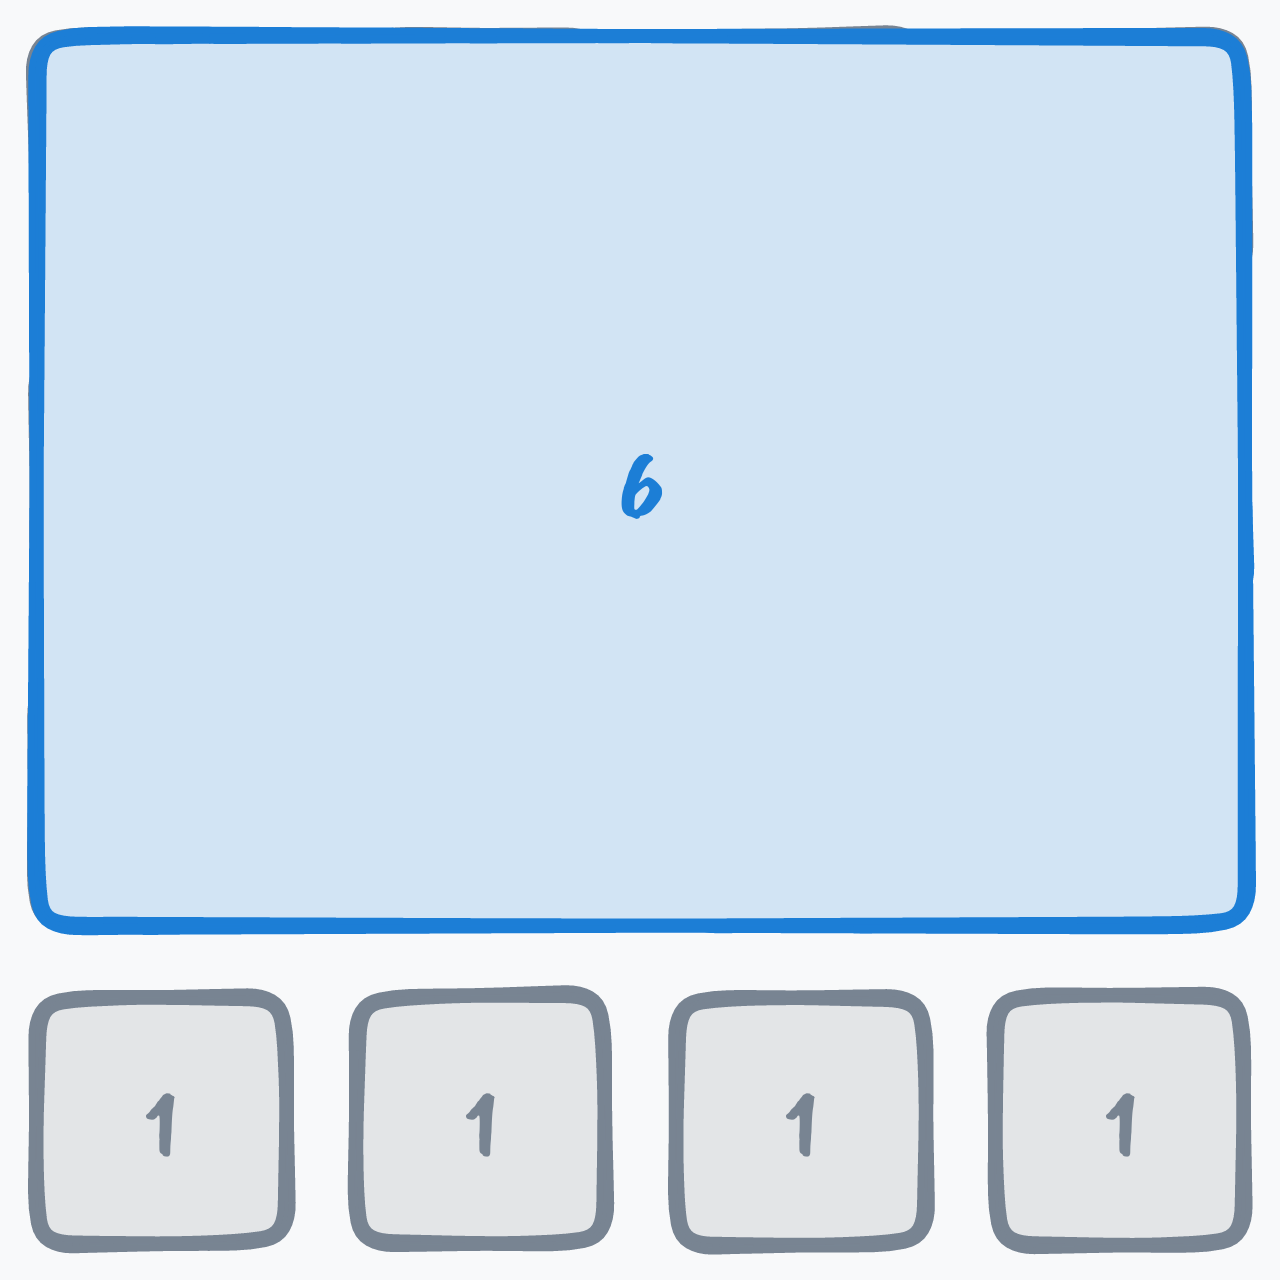
\includegraphics[width=6.0cm]{img/img_12.png}
        \item 先把最大的問題加起來
    \end{itemize}
\end{frame}

\begin{frame}
    \frametitle{額外問題}
    \begin{itemize}
        \item 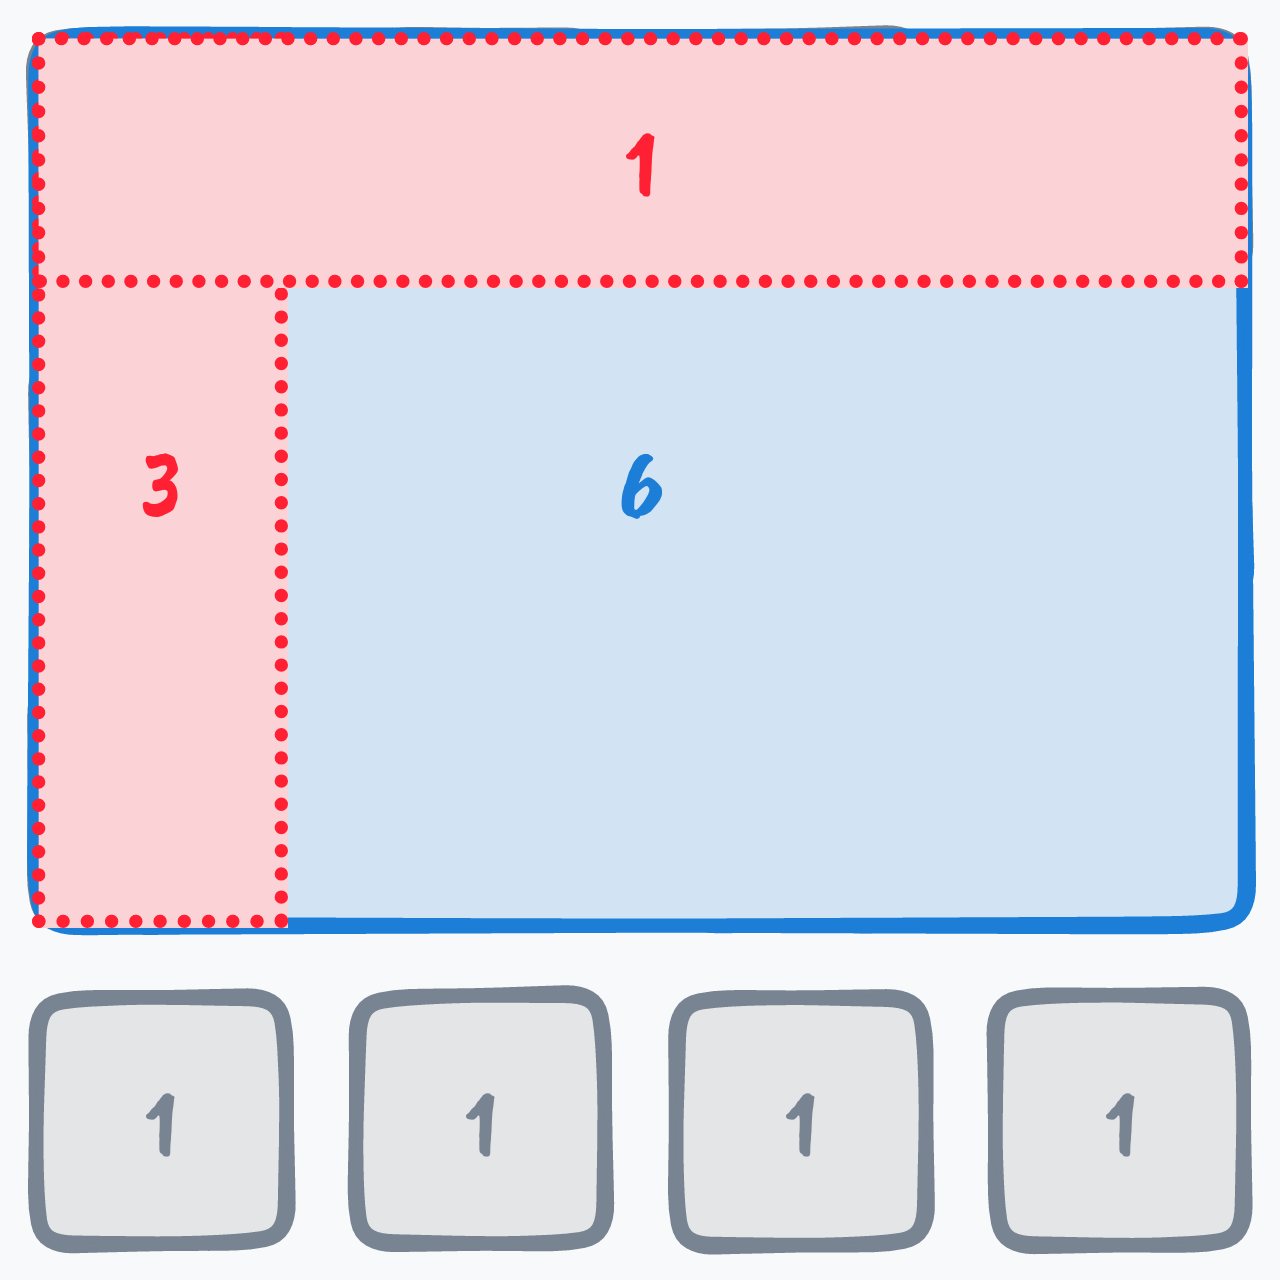
\includegraphics[width=6.0cm]{img/img_13.png}
        \item 將不需要的範圍刪除
    \end{itemize}
\end{frame}

\begin{frame}
    \frametitle{額外問題}
    \begin{itemize}
        \item 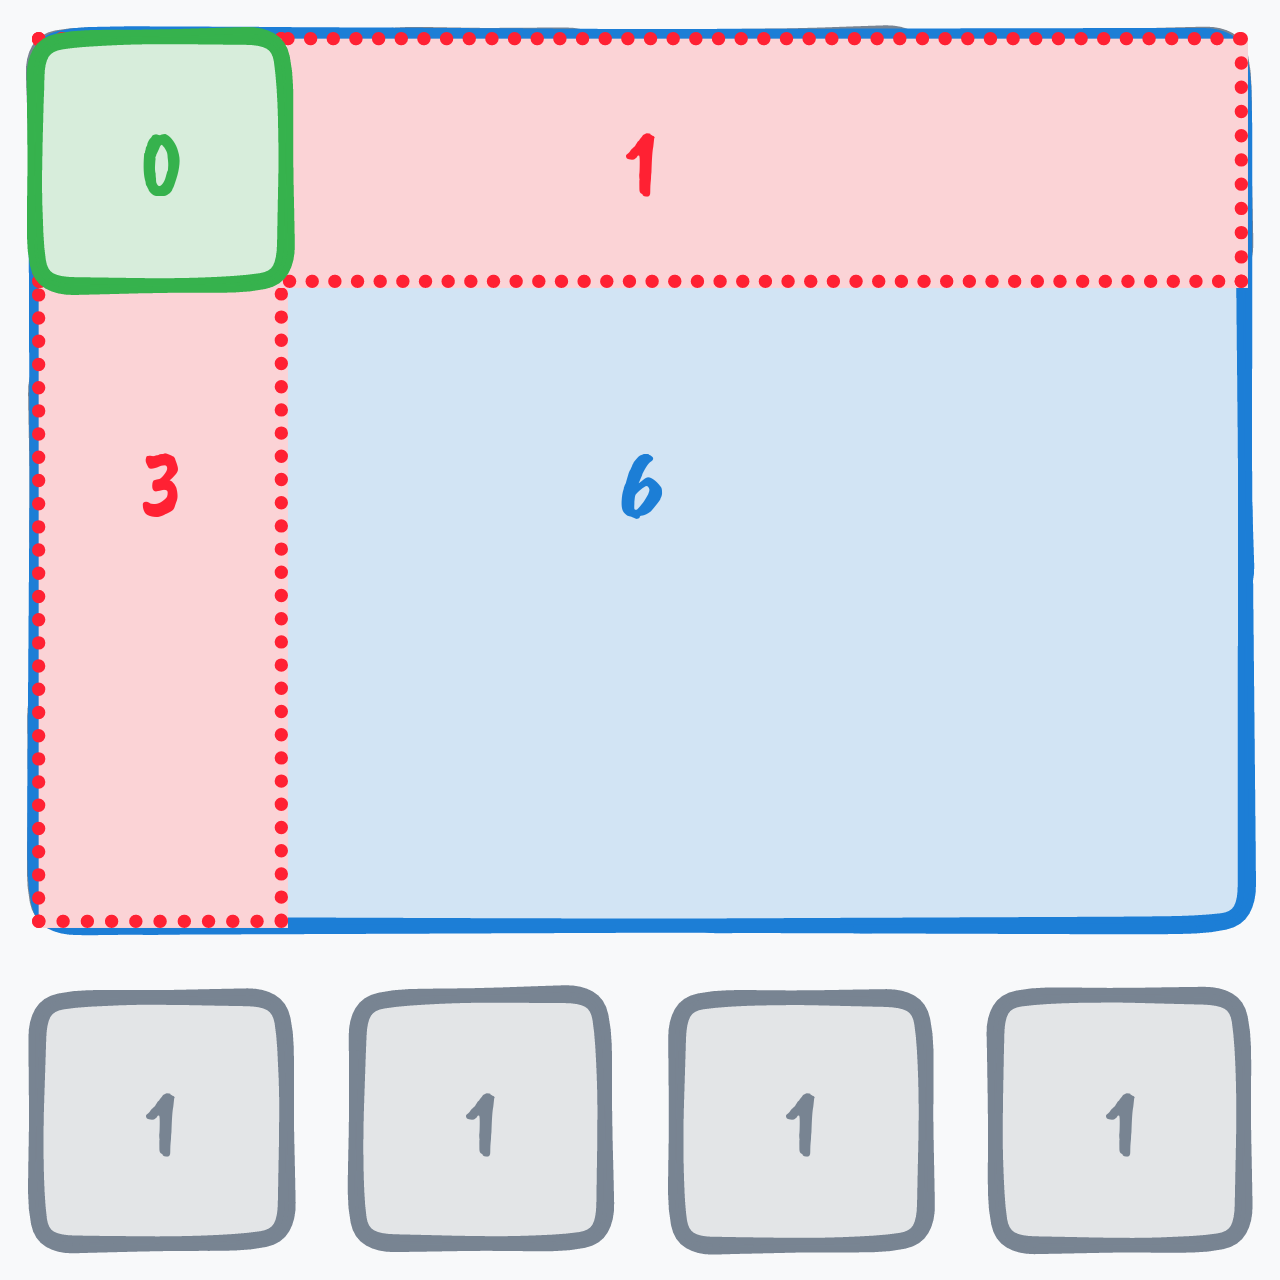
\includegraphics[width=6.0cm]{img/img_14.png}
        \item 把多刪除的範圍加回去
    \end{itemize}
\end{frame}

\end{document}